\chapter{Pyramus and Thisbe}

About two-thirds of the way along the Faubourg Saint-Honoré, and in the
rear of one of the most imposing mansions in this rich neighborhood,
where the various houses vie with each other for elegance of design and
magnificence of construction, extended a large garden, where the
wide-spreading chestnut-trees raised their heads high above the walls
in a solid rampart, and with the coming of every spring scattered a
shower of delicate pink and white blossoms into the large stone vases
that stood upon the two square pilasters of a curiously wrought iron
gate, that dated from the time of Louis XIII.

This noble entrance, however, in spite of its striking appearance and
the graceful effect of the geraniums planted in the two vases, as they
waved their variegated leaves in the wind and charmed the eye with
their scarlet bloom, had fallen into utter disuse. The proprietors of
the mansion had many years before thought it best to confine themselves
to the possession of the house itself, with its thickly planted
courtyard, opening into the Faubourg Saint-Honoré, and to the garden
shut in by this gate, which formerly communicated with a fine
kitchen-garden of about an acre. For the demon of speculation drew a
line, or in other words projected a street, at the farther side of the
kitchen-garden. The street was laid out, a name was chosen and posted
up on an iron plate, but before construction was begun, it occurred to
the possessor of the property that a handsome sum might be obtained for
the ground then devoted to fruits and vegetables, by building along the
line of the proposed street, and so making it a branch of communication
with the Faubourg Saint-Honoré itself, one of the most important
thoroughfares in the city of Paris.

In matters of speculation, however, though “man proposes,” yet “money
disposes.” From some such difficulty the newly named street died almost
in birth, and the purchaser of the kitchen-garden, having paid a high
price for it, and being quite unable to find anyone willing to take his
bargain off his hands without a considerable loss, yet still clinging
to the belief that at some future day he should obtain a sum for it
that would repay him, not only for his past outlay, but also the
interest upon the capital locked up in his new acquisition, contented
himself with letting the ground temporarily to some market-gardeners,
at a yearly rental of 500 francs.

And so, as we have said, the iron gate leading into the kitchen-garden
had been closed up and left to the rust, which bade fair before long to
eat off its hinges, while to prevent the ignoble glances of the diggers
and delvers of the ground from presuming to sully the aristocratic
enclosure belonging to the mansion, the gate had been boarded up to a
height of six feet. True, the planks were not so closely adjusted but
that a hasty peep might be obtained through their interstices; but the
strict decorum and rigid propriety of the inhabitants of the house left
no grounds for apprehending that advantage would be taken of that
circumstance.

Horticulture seemed, however, to have been abandoned in the deserted
kitchen-garden; and where cabbages, carrots, radishes, peas, and melons
had once flourished, a scanty crop of lucern alone bore evidence of its
being deemed worthy of cultivation. A small, low door gave egress from
the walled space we have been describing into the projected street, the
ground having been abandoned as unproductive by its various renters,
and had now fallen so completely in general estimation as to return not
even the one-half per cent it had originally paid. Towards the house
the chestnut-trees we have before mentioned rose high above the wall,
without in any way affecting the growth of other luxuriant shrubs and
flowers that eagerly dressed forward to fill up the vacant spaces, as
though asserting their right to enjoy the boon of light and air. At one
corner, where the foliage became so thick as almost to shut out day, a
large stone bench and sundry rustic seats indicated that this sheltered
spot was either in general favor or particular use by some inhabitant
of the house, which was faintly discernible through the dense mass of
verdure that partially concealed it, though situated but a hundred
paces off.

Whoever had selected this retired portion of the grounds as the
boundary of a walk, or as a place for meditation, was abundantly
justified in the choice by the absence of all glare, the cool,
refreshing shade, the screen it afforded from the scorching rays of the
sun, that found no entrance there even during the burning days of
hottest summer, the incessant and melodious warbling of birds, and the
entire removal from either the noise of the street or the bustle of the
mansion. On the evening of one of the warmest days spring had yet
bestowed on the inhabitants of Paris, might be seen negligently thrown
upon the stone bench, a book, a parasol, and a work-basket, from which
hung a partly embroidered cambric handkerchief, while at a little
distance from these articles was a young woman, standing close to the
iron gate, endeavoring to discern something on the other side by means
of the openings in the planks,—the earnestness of her attitude and the
fixed gaze with which she seemed to seek the object of her wishes,
proving how much her feelings were interested in the matter.

At that instant the little side-gate leading from the waste ground to
the street was noiselessly opened, and a tall, powerful young man
appeared. He was dressed in a common gray blouse and velvet cap, but
his carefully arranged hair, beard and moustache, all of the richest
and glossiest black, ill accorded with his plebeian attire. After
casting a rapid glance around him, in order to assure himself that he
was unobserved, he entered by the small gate, and, carefully closing
and securing it after him, proceeded with a hurried step towards the
barrier.

At the sight of him she expected, though probably not in such a
costume, the young woman started in terror, and was about to make a
hasty retreat. But the eye of love had already seen, even through the
narrow chinks of the wooden palisades, the movement of the white robe,
and observed the fluttering of the blue sash. Pressing his lips close
to the planks, he exclaimed:

“Don’t be alarmed, Valentine—it is I!”

Again the timid girl found courage to return to the gate, saying, as
she did so:

“And why do you come so late today? It is almost dinner-time, and I had
to use no little diplomacy to get rid of my watchful stepmother, my
too-devoted maid, and my troublesome brother, who is always teasing me
about coming to work at my embroidery, which I am in a fair way never
to get done. So pray excuse yourself as well as you can for having made
me wait, and, after that, tell me why I see you in a dress so singular
that at first I did not recognize you.”

“Dearest Valentine,” said the young man, “the difference between our
respective stations makes me fear to offend you by speaking of my love,
but yet I cannot find myself in your presence without longing to pour
forth my soul, and tell you how fondly I adore you. If it be but to
carry away with me the recollection of such sweet moments, I could even
thank you for chiding me, for it leaves me a gleam of hope, that if you
did not expect me (and that indeed would be worse than vanity to
suppose), at least I was in your thoughts. You asked me the cause of my
being late, and why I come disguised. I will candidly explain the
reason of both, and I trust to your goodness to pardon me. I have
chosen a trade.”

“A trade? Oh, Maximilian, how can you jest at a time when we have such
deep cause for uneasiness?”

“Heaven keep me from jesting with that which is far dearer to me than
life itself! But listen to me, Valentine, and I will tell you all about
it. I became weary of ranging fields and scaling walls, and seriously
alarmed at the idea suggested by you, that if caught hovering about
here your father would very likely have me sent to prison as a thief.
That would compromise the honor of the French army, to say nothing of
the fact that the continual presence of a captain of Spahis in a place
where no warlike projects could be supposed to account for it might
well create surprise; so I have become a gardener, and, consequently,
adopted the costume of my calling.”

“What excessive nonsense you talk, Maximilian!”

“Nonsense? Pray do not call what I consider the wisest action of my
life by such a name. Consider, by becoming a gardener I effectually
screen our meetings from all suspicion or danger.”

\begin{figure}[ht]
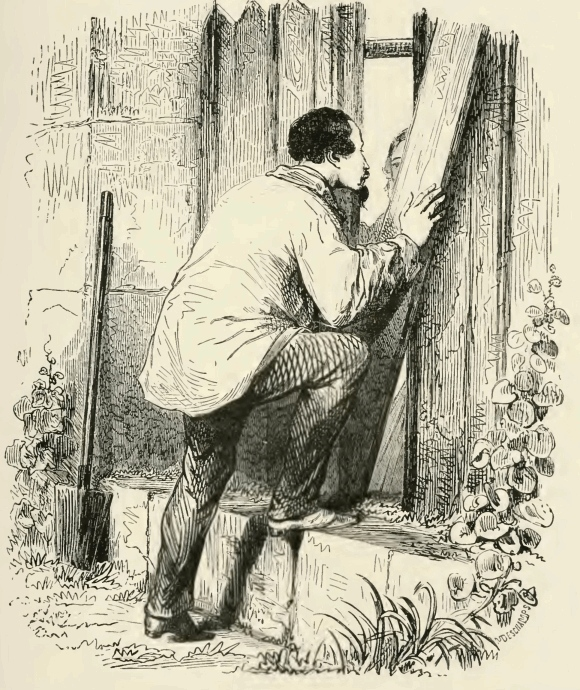
\includegraphics[width=\textwidth]{30053m.jpg}
\end{figure}

“I beseech of you, Maximilian, to cease trifling, and tell me what you
really mean.”

“Simply, that having ascertained that the piece of ground on which I
stand was to let, I made application for it, was readily accepted by
the proprietor, and am now master of this fine crop of lucern. Think of
that, Valentine! There is nothing now to prevent my building myself a
little hut on my plantation, and residing not twenty yards from you.
Only imagine what happiness that would afford me. I can scarcely
contain myself at the bare idea. Such felicity seems above all price—as
a thing impossible and unattainable. But would you believe that I
purchase all this delight, joy, and happiness, for which I would
cheerfully have surrendered ten years of my life, at the small cost of
500 francs per annum, paid quarterly? Henceforth we have nothing to
fear. I am on my own ground, and have an undoubted right to place a
ladder against the wall, and to look over when I please, without having
any apprehensions of being taken off by the police as a suspicious
character. I may also enjoy the precious privilege of assuring you of
my fond, faithful, and unalterable affection, whenever you visit your
favorite bower, unless, indeed, it offends your pride to listen to
professions of love from the lips of a poor workingman, clad in a
blouse and cap.”

A faint cry of mingled pleasure and surprise escaped from the lips of
Valentine, who almost instantly said, in a saddened tone, as though
some envious cloud darkened the joy which illumined her heart:

“Alas, no, Maximilian, this must not be, for many reasons. We should
presume too much on our own strength, and, like others, perhaps, be led
astray by our blind confidence in each other’s prudence.”

“How can you for an instant entertain so unworthy a thought, dear
Valentine? Have I not, from the first blessed hour of our acquaintance,
schooled all my words and actions to your sentiments and ideas? And you
have, I am sure, the fullest confidence in my honor. When you spoke to
me of experiencing a vague and indefinite sense of coming danger, I
placed myself blindly and devotedly at your service, asking no other
reward than the pleasure of being useful to you; and have I ever since,
by word or look, given you cause of regret for having selected me from
the numbers that would willingly have sacrificed their lives for you?
You told me, my dear Valentine, that you were engaged to M. d’Épinay,
and that your father was resolved upon completing the match, and that
from his will there was no appeal, as M. de Villefort was never known
to change a determination once formed. I kept in the background, as you
wished, and waited, not for the decision of your heart or my own, but
hoping that Providence would graciously interpose in our behalf, and
order events in our favor. But what cared I for delays or difficulties,
Valentine, as long as you confessed that you loved me, and took pity on
me? If you will only repeat that avowal now and then, I can endure
anything.”

“Ah, Maximilian, that is the very thing that makes you so bold, and
which renders me at once so happy and unhappy, that I frequently ask
myself whether it is better for me to endure the harshness of my
stepmother, and her blind preference for her own child, or to be, as I
now am, insensible to any pleasure save such as I find in these
meetings, so fraught with danger to both.”

“I will not admit that word,” returned the young man; “it is at once
cruel and unjust. Is it possible to find a more submissive slave than
myself? You have permitted me to converse with you from time to time,
Valentine, but forbidden my ever following you in your walks or
elsewhere—have I not obeyed? And since I found means to enter this
enclosure to exchange a few words with you through this gate—to be
close to you without really seeing you—have I ever asked so much as to
touch the hem of your gown or tried to pass this barrier which is but a
trifle to one of my youth and strength? Never has a complaint or a
murmur escaped me. I have been bound by my promises as rigidly as any
knight of olden times. Come, come, dearest Valentine, confess that what
I say is true, lest I be tempted to call you unjust.”

\begin{figure}[ht]
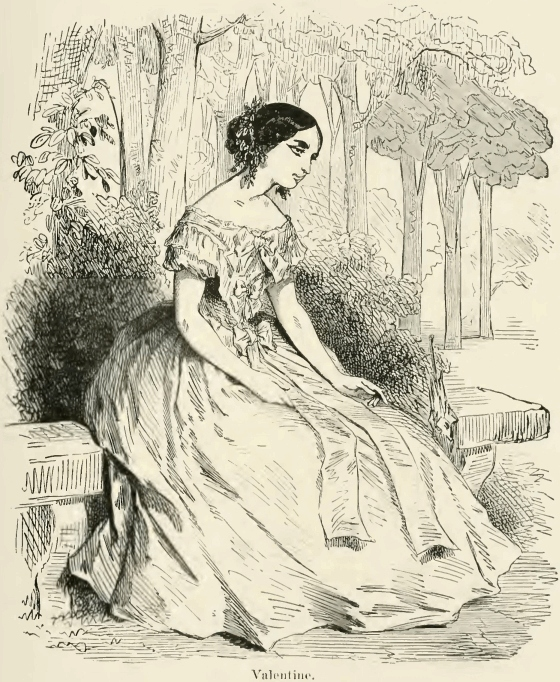
\includegraphics[width=\textwidth]{30055m.jpg}
\end{figure}

“It is true,” said Valentine, as she passed the end of her slender
fingers through a small opening in the planks, and permitted Maximilian
to press his lips to them, “and you are a true and faithful friend; but
still you acted from motives of self-interest, my dear Maximilian, for
you well knew that from the moment in which you had manifested an
opposite spirit all would have been ended between us. You promised to
bestow on me the friendly affection of a brother. For I have no friend
but yourself upon earth, who am neglected and forgotten by my father,
harassed and persecuted by my stepmother, and left to the sole
companionship of a paralyzed and speechless old man, whose withered
hand can no longer press mine, and who can speak to me with the eye
alone, although there still lingers in his heart the warmest tenderness
for his poor grandchild. Oh, how bitter a fate is mine, to serve either
as a victim or an enemy to all who are stronger than myself, while my
only friend and supporter is a living corpse! Indeed, indeed,
Maximilian, I am very miserable, and if you love me it must be out of
pity.”

“Valentine,” replied the young man, deeply affected, “I will not say
you are all I love in the world, for I dearly prize my sister and
brother-in-law; but my affection for them is calm and tranquil, in no
manner resembling what I feel for you. When I think of you my heart
beats fast, the blood burns in my veins, and I can hardly breathe; but
I solemnly promise you to restrain all this ardor, this fervor and
intensity of feeling, until you yourself shall require me to render
them available in serving or assisting you. M. Franz is not expected to
return home for a year to come, I am told; in that time many favorable
and unforeseen chances may befriend us. Let us, then, hope for the
best; hope is so sweet a comforter. Meanwhile, Valentine, while
reproaching me with selfishness, think a little what you have been to
me—the beautiful but cold resemblance of a marble Venus. What promise
of future reward have you made me for all the submission and obedience
I have evinced?—none whatever. What granted me?—scarcely more. You tell
me of M. Franz d’Épinay, your betrothed lover, and you shrink from the
idea of being his wife; but tell me, Valentine, is there no other
sorrow in your heart? You see me devoted to you, body and soul, my life
and each warm drop that circles round my heart are consecrated to your
service; you know full well that my existence is bound up in yours—that
were I to lose you I would not outlive the hour of such crushing
misery; yet you speak with calmness of the prospect of your being the
wife of another! Oh, Valentine, were I in your place, and did I feel
conscious, as you do, of being worshipped, adored, with such a love as
mine, a hundred times at least should I have passed my hand between
these iron bars, and said, ‘Take this hand, dearest Maximilian, and
believe that, living or dead, I am yours—yours only, and forever!’”

The poor girl made no reply, but her lover could plainly hear her sobs
and tears. A rapid change took place in the young man’s feelings.

“Dearest, dearest Valentine,” exclaimed he, “forgive me if I have
offended you, and forget the words I spoke if they have unwittingly
caused you pain.”

“No, Maximilian, I am not offended,” answered she, “but do you not see
what a poor, helpless being I am, almost a stranger and an outcast in
my father’s house, where even he is seldom seen; whose will has been
thwarted, and spirits broken, from the age of ten years, beneath the
iron rod so sternly held over me; oppressed, mortified, and persecuted,
day by day, hour by hour, minute by minute, no person has cared for,
even observed my sufferings, nor have I ever breathed one word on the
subject save to yourself. Outwardly and in the eyes of the world, I am
surrounded by kindness and affection; but the reverse is the case. The
general remark is, ‘Oh, it cannot be expected that one of so stern a
character as M. Villefort could lavish the tenderness some fathers do
on their daughters. What though she has lost her own mother at a tender
age, she has had the happiness to find a second mother in Madame de
Villefort.’ The world, however, is mistaken; my father abandons me from
utter indifference, while my stepmother detests me with a hatred so
much the more terrible because it is veiled beneath a continual smile.”

“Hate you, sweet Valentine,” exclaimed the young man; “how is it
possible for anyone to do that?”

“Alas,” replied the weeping girl, “I am obliged to own that my
stepmother’s aversion to me arises from a very natural source—her
overweening love for her own child, my brother Edward.”

“But why should it?”

“I do not know; but, though unwilling to introduce money matters into
our present conversation, I will just say this much—that her extreme
dislike to me has its origin there; and I much fear she envies me the
fortune I enjoy in right of my mother, and which will be more than
doubled at the death of M. and Mme. de Saint-Méran, whose sole heiress
I am. Madame de Villefort has nothing of her own, and hates me for
being so richly endowed. Alas, how gladly would I exchange the half of
this wealth for the happiness of at least sharing my father’s love. God
knows, I would prefer sacrificing the whole, so that it would obtain me
a happy and affectionate home.”

“Poor Valentine!”

“I seem to myself as though living a life of bondage, yet at the same
time am so conscious of my own weakness that I fear to break the
restraint in which I am held, lest I fall utterly helpless. Then, too,
my father is not a person whose orders may be infringed with impunity;
protected as he is by his high position and firmly established
reputation for talent and unswerving integrity, no one could oppose
him; he is all-powerful even with the king; he would crush you at a
word. Dear Maximilian, believe me when I assure you that if I do not
attempt to resist my father’s commands it is more on your account than
my own.”

“But why, Valentine, do you persist in anticipating the worst,—why
picture so gloomy a future?”

“Because I judge it from the past.”

“Still, consider that although I may not be, strictly speaking, what is
termed an illustrious match for you, I am, for many reasons, not
altogether so much beneath your alliance. The days when such
distinctions were so nicely weighed and considered no longer exist in
France, and the first families of the monarchy have intermarried with
those of the empire. The aristocracy of the lance has allied itself
with the nobility of the cannon. Now I belong to this last-named class;
and certainly my prospects of military preferment are most encouraging
as well as certain. My fortune, though small, is free and unfettered,
and the memory of my late father is respected in our country,
Valentine, as that of the most upright and honorable merchant of the
city; I say our country, because you were born not far from
Marseilles.”

“Don’t speak of Marseilles, I beg of you, Maximilian; that one word
brings back my mother to my recollection—my angel mother, who died too
soon for myself and all who knew her; but who, after watching over her
child during the brief period allotted to her in this world, now, I
fondly hope, watches from her home in heaven. Oh, if my mother were
still living, there would be nothing to fear, Maximilian, for I would
tell her that I loved you, and she would protect us.”

“I fear, Valentine,” replied the lover, “that were she living I should
never have had the happiness of knowing you; you would then have been
too happy to have stooped from your grandeur to bestow a thought on
me.”

“Now it is you who are unjust, Maximilian,” cried Valentine; “but there
is one thing I wish to know.”

“And what is that?” inquired the young man, perceiving that Valentine
hesitated.

“Tell me truly, Maximilian, whether in former days, when our fathers
dwelt at Marseilles, there was ever any misunderstanding between them?”

“Not that I am aware of,” replied the young man, “unless, indeed, any
ill-feeling might have arisen from their being of opposite parties—your
father was, as you know, a zealous partisan of the Bourbons, while mine
was wholly devoted to the emperor; there could not possibly be any
other difference between them. But why do you ask?”

“I will tell you,” replied the young girl, “for it is but right you
should know. Well, on the day when your appointment as an officer of
the Legion of Honor was announced in the papers, we were all sitting
with my grandfather, M. Noirtier; M. Danglars was there also—you
recollect M. Danglars, do you not, Maximilian, the banker, whose horses
ran away with my stepmother and little brother, and very nearly killed
them? While the rest of the company were discussing the approaching
marriage of Mademoiselle Danglars, I was reading the paper to my
grandfather; but when I came to the paragraph about you, although I had
done nothing else but read it over to myself all the morning (you know
you had told me all about it the previous evening), I felt so happy,
and yet so nervous, at the idea of speaking your name aloud, and before
so many people, that I really think I should have passed it over, but
for the fear that my doing so might create suspicions as to the cause
of my silence; so I summoned up all my courage, and read it as firmly
and as steadily as I could.”

\begin{figure}[ht]
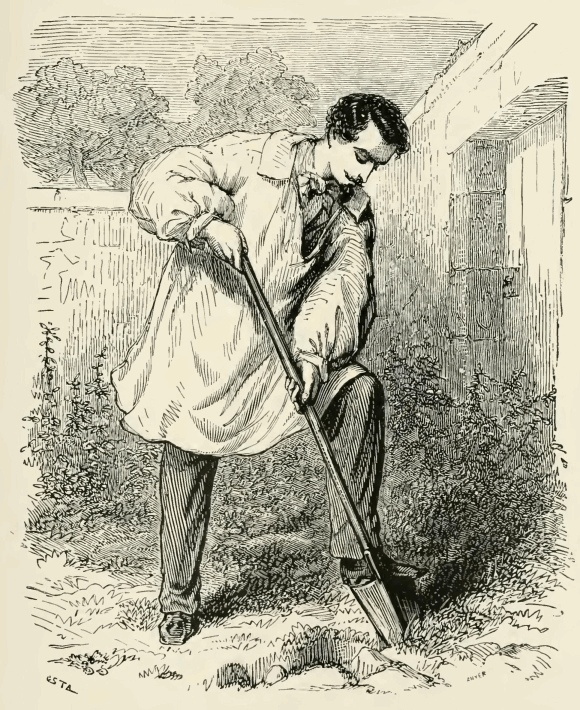
\includegraphics[width=\textwidth]{30059m.jpg}
\end{figure}

“Dear Valentine!”

“Well, would you believe it? directly my father caught the sound of
your name he turned round quite hastily, and, like a poor silly thing,
I was so persuaded that everyone must be as much affected as myself by
the utterance of your name, that I was not surprised to see my father
start, and almost tremble; but I even thought (though that surely must
have been a mistake) that M. Danglars trembled too.”

“‘Morrel, Morrel,’ cried my father, ‘stop a bit;’ then knitting his
brows into a deep frown, he added, ‘surely this cannot be one of the
Morrel family who lived at Marseilles, and gave us so much trouble from
their violent Bonapartism—I mean about the year 1815.’

“‘Yes,’ replied M. Danglars, ‘I believe he is the son of the old
shipowner.’”

“Indeed,” answered Maximilian; “and what did your father say then,
Valentine?”

“Oh, such a dreadful thing, that I don’t dare to tell you.”

“Always tell me everything,” said Maximilian with a smile.

“‘Ah,’ continued my father, still frowning, ‘their idolized emperor
treated these madmen as they deserved; he called them ‘food for
cannon,’ which was precisely all they were good for; and I am delighted
to see that the present government have adopted this salutary principle
with all its pristine vigor; if Algiers were good for nothing but to
furnish the means of carrying so admirable an idea into practice, it
would be an acquisition well worthy of struggling to obtain. Though it
certainly does cost France somewhat dear to assert her rights in that
uncivilized country.’”

“Brutal politics, I must confess.” said Maximilian; “but don’t attach
any serious importance, dear, to what your father said. My father was
not a bit behind yours in that sort of talk. ‘Why,’ said he, ‘does not
the emperor, who has devised so many clever and efficient modes of
improving the art of war, organize a regiment of lawyers, judges and
legal practitioners, sending them in the hottest fire the enemy could
maintain, and using them to save better men?’ You see, my dear, that
for picturesque expression and generosity of spirit there is not much
to choose between the language of either party. But what did M.
Danglars say to this outburst on the part of the procureur?”

“Oh, he laughed, and in that singular manner so peculiar to
himself—half-malicious, half-ferocious; he almost immediately got up
and took his leave; then, for the first time, I observed the agitation
of my grandfather, and I must tell you, Maximilian, that I am the only
person capable of discerning emotion in his paralyzed frame. And I
suspected that the conversation that had been carried on in his
presence (for they always say and do what they like before the dear old
man, without the smallest regard for his feelings) had made a strong
impression on his mind; for, naturally enough, it must have pained him
to hear the emperor he so devotedly loved and served spoken of in that
depreciating manner.”

“The name of M. Noirtier,” interposed Maximilian, “is celebrated
throughout Europe; he was a statesman of high standing, and you may or
may not know, Valentine, that he took a leading part in every
Bonapartist conspiracy set on foot during the restoration of the
Bourbons.”

“Oh, I have often heard whispers of things that seem to me most
strange—the father a Bonapartist, the son a Royalist; what can have
been the reason of so singular a difference in parties and politics?
But to resume my story; I turned towards my grandfather, as though to
question him as to the cause of his emotion; he looked expressively at
the newspaper I had been reading. ‘What is the matter, dear
grandfather?’ said I, ‘are you pleased?’ He gave me a sign in the
affirmative. ‘With what my father said just now?’ He returned a sign in
the negative. ‘Perhaps you liked what M. Danglars said?’ Another sign
in the negative. ‘Oh, then, you were glad to hear that M. Morrel (I
didn’t dare to say Maximilian) had been made an officer of the Legion
of Honor?’ He signified assent; only think of the poor old man’s being
so pleased to think that you, who were a perfect stranger to him, had
been made an officer of the Legion of Honor! Perhaps it was a mere whim
on his part, for he is falling, they say, into second childhood, but I
love him for showing so much interest in you.”

“How singular,” murmured Maximilian; “your father hates me, while your
grandfather, on the contrary—What strange feelings are aroused by
politics.”

“Hush,” cried Valentine, suddenly; “someone is coming!” Maximilian
leaped at one bound into his crop of lucern, which he began to pull up
in the most ruthless way, under the pretext of being occupied in
weeding it.

“Mademoiselle, mademoiselle!” exclaimed a voice from behind the trees.
“Madame is searching for you everywhere; there is a visitor in the
drawing-room.”

“A visitor?” inquired Valentine, much agitated; “who is it?”

“Some grand personage—a prince I believe they said—the Count of Monte
Cristo.”

“I will come directly,” cried Valentine aloud.

The name of Monte Cristo sent an electric shock through the young man
on the other side of the iron gate, to whom Valentine’s \textit{“I am coming”}
was the customary signal of farewell.

“Now, then,” said Maximilian, leaning on the handle of his spade, “I
would give a good deal to know how it comes about that the Count of
Monte Cristo is acquainted with M. de Villefort.”
